\chapter{Beyond Words: The Development of Feature Sparsity} \label{chapter:sparsity}

\epigraph{``In this box are all the words I know,'' he said. ``Most of them you will never need, some you will use constantly, but with them you may ask all the questions which have never been answered and answer all the questions which have never been asked.''
}{Norton Juster, \textit{The Phantom Tollbooth}}
% \epigraph{``It will take years to collect all those sounds again,'' she sobbed, ``and even longer to put them back in proper order. But it's all my fault. For you can't improve sound by having only silence. The problem is to use each at the proper time.''}{Norton Juster, \textit{The Phantom Tollbooth}}

In Chapters \ref{chapter:svcca} and \ref{chapter:interdependence}, we explored the temporal dynamics of models acquiring linguistic structure as training progresses. Here we turn to investigate more abstract properties of representations and how they evolve. In particular, the following work explores how \textbf{feature sparsity} naturally emerges in LMs during training. 

Rather than consider the gradual development of hierarchical syntactic structure, we observe the dispersal or concentration (i.e., sparsity) of intermediate vector representations as a simple function of the frequency and predictability of each word. We better characterize the relationship between word frequency and the distribution of its ``storage'' in a model. The time dimension is essential to understanding the contributing factors to sparsity, because the model is more exposed to a word the longer it trains for, as well as in response to the word's corpus frequency. 

As well as providing consideration of this crucial confounding factor between word frequency and a model's exposure to a word, viewing the time course of training again offers additional insights. We see how gradients responding to a word become sparser--meaning salient information is localized to a few neurons--as a network is exposed more to that word. This validates work that considers individual neurons rather than entire subspaces \citep{hennigen_intrinsic_2020,durrani_analyzing_2020,dalvi_what_2018}. We see that LSTM layers quickly correlate word frequency and sparsity, before the embedding layer surpasses the LSTMs in developing this correlation. The patterns we observe are, as in Chapter~\ref{chapter:svcca}'s discussion of the Information Bottleneck Hypothesis, possibly linked to a memorize/compress phase shift. 


\paragraph*{Publication Status } This work was published in the Identifying and Understanding Deep Learning Phenomena Workshop at ICML 2019.


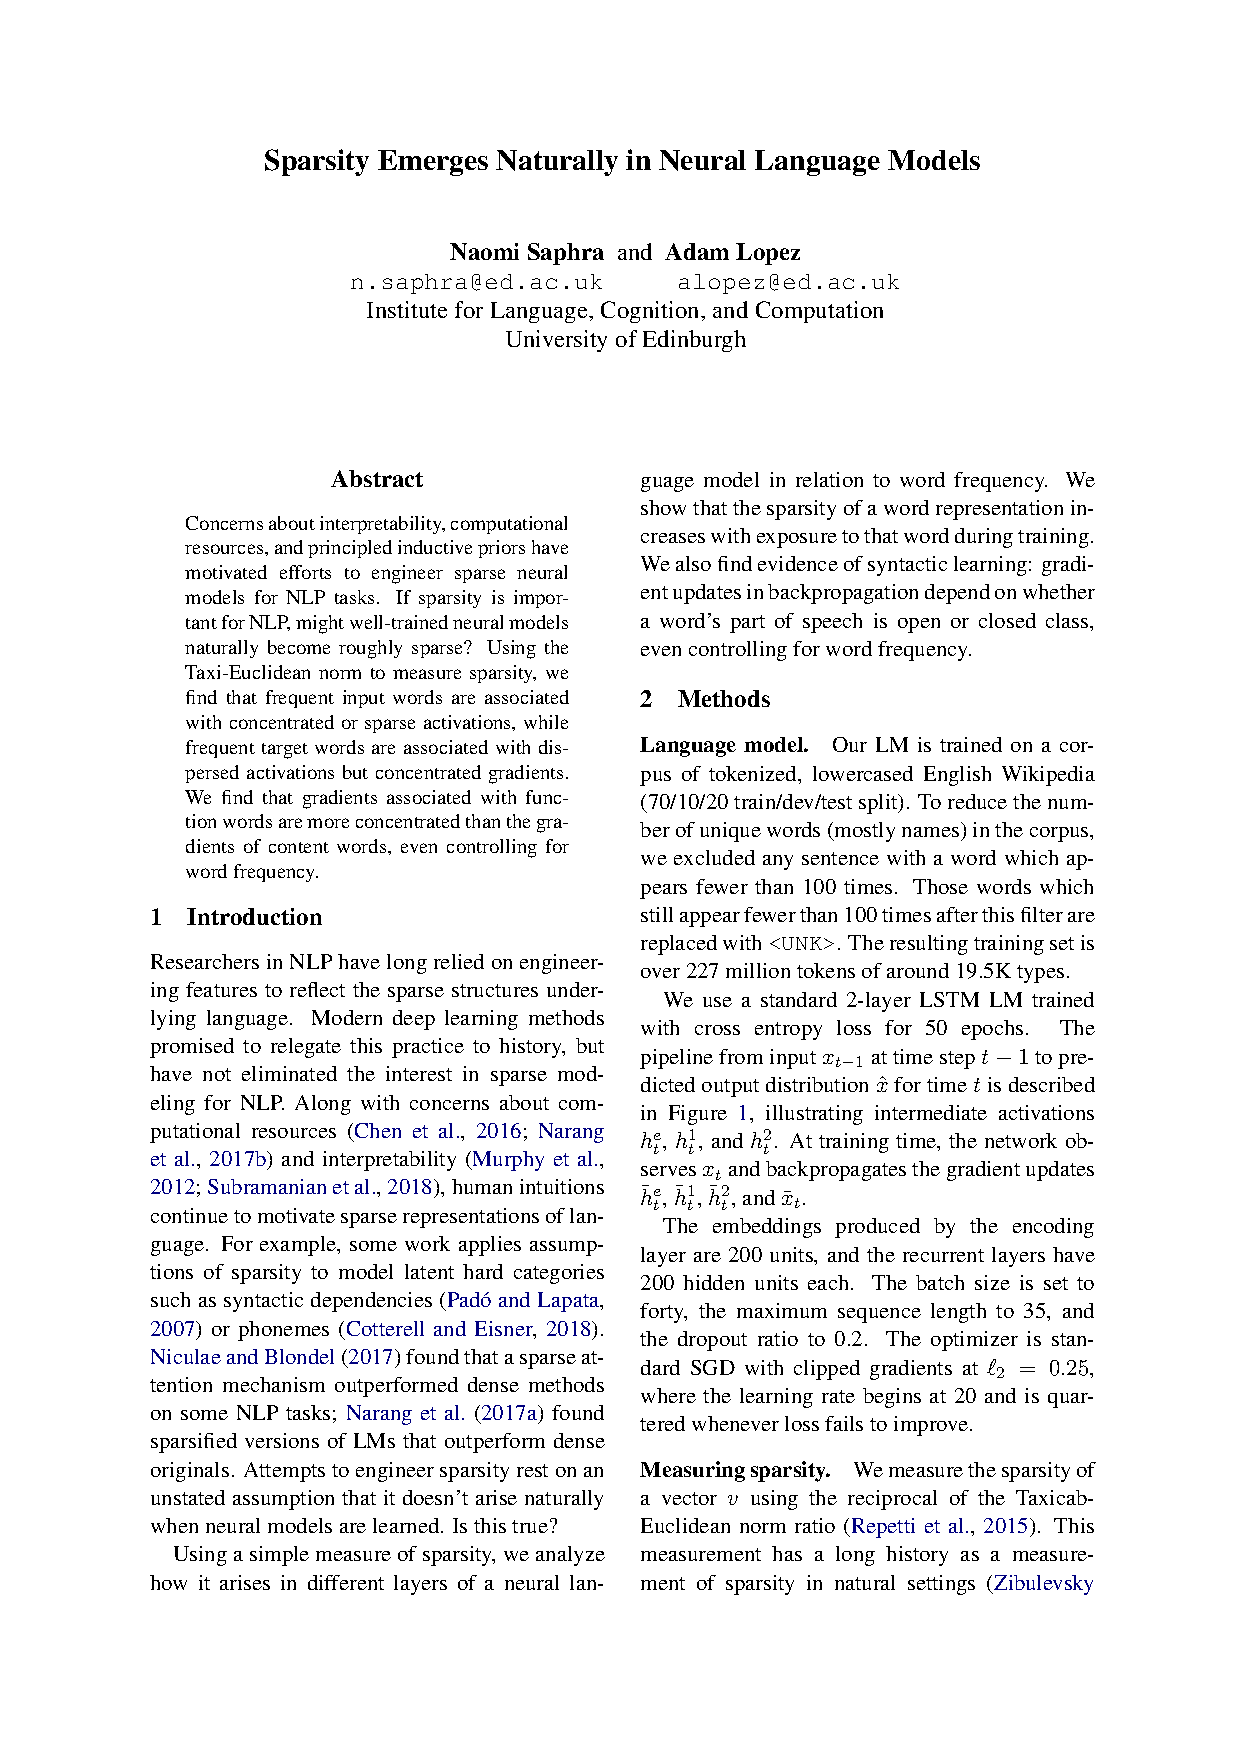
\includepdf[pages=-,pagecommand={}]{sparsity/chapter.pdf}

\section{Comments on the Paper}

In this paper, we have investigated the sparsity of activations and, using the same sparsity metric applied to gradients, observed how localized change is across neurons. 

\subsection{Localization of Changes}

The local loss surface revealed by gradients is not the only way of viewing change across neurons. Because the optimizer does not follow this surface perfectly, and the training data is not the only way of viewing change in error, we may want to investigate change in each neuron through \textbf{Loss Change Allocation} (LCA)~\citep{lan_lca:_2019}.

\subsubsection{Loss Change Allocation} \label{sec:lca}

LCA is a method that does not look directly at the gradient with respect to training error, but instead allocates responsibility for \textit{actual} error change after a training step.

If we consider the loss function over a training set $L(\theta_t)$ with the parameters at timestep~$t$, LCA is based on a first order Taylor approximation of the path between two timesteps:
\begin{align}
    L(\theta_{t+1}) - L(\theta_t) &= \int_{\theta_t}^{\theta_{t+1}} <\nabla_{\theta} L(\theta_t), d \theta>\\
    & \approx < \nabla_\theta L(\theta_t), \theta_{t+1} - \theta_t>
\end{align}

This dot product can be reformulated into an element-wise operation, such that we can consider the individual parameters that contribute to this change in loss. We therefore define the LCA allocated to parameter unit $\theta^{(i)}$ like so:
\begin{equation}
    \sum_{i=0}^{K-1} A_{t,i} = \sum_{i=0}^{K-1} (\nabla_{\theta} L(\theta_t))^{(i)} (\theta_{t+1}^{(i)} - \theta_t^{(i)})
\end{equation}
This way, we could consider whether following the gradient in a particular direction actually leads to a particular unit improving or damaging performance when considered in combination with the other changes made during that timestep. 

Using LCA, \citet{lan_lca:_2019} found that only a little over half of parameters actually help improve performance in their changes at any given time step, with some entire layers moving against the gradient in a particular timestep and damaging performance. Because all layers tend to move in synchrony, they hypothesize that these damaging layers lag behind others while they oscillate back and forth over valleys in the optimization landscape, therefore moving against the overall gradient motion. These dynamics calls into question a simplistic view of the training process through the lens of the gradient landscape itself. Even from timestep to timestep, the movement of parameters along the gradient does not translate directly to improvement in the training objective.

\subsection{Generalizing to Attentional Models}

Current Transformer models provide new motivations and methods for considering sparsity during the forward pass through a neural network. Attention distributions can be easily measured in terms of their entropy, which offers additional information about how localized word importance itself might be, as it gives a view of how sparse \textit{attention} naturally is across words.